\subsection{センサネットワーク展開時のグループ化}
センサネットワークが展開される初回起動時にグループを作成する手法を述べる.下記図\ref{fig:group_on_activation}にシーケンスを示す.GWがセンサノードのトポロジを把握するため,各ノードが周囲のノード情報を探索する.ノードは起動時に,BLEで自身の情報を発信するとともに,周囲のノード情報を収集し近傍ノードのリストを作成した後,NSへ送信する.GWがノード情報を集約した後,グループとGL を選出する.GWはノードの固有ID,及び個々の信号強度を用いて重複ノードのないグループを作成しグループごとに1つGL ノードを選出する.

\begin{figure}[]
    \begin{center}
    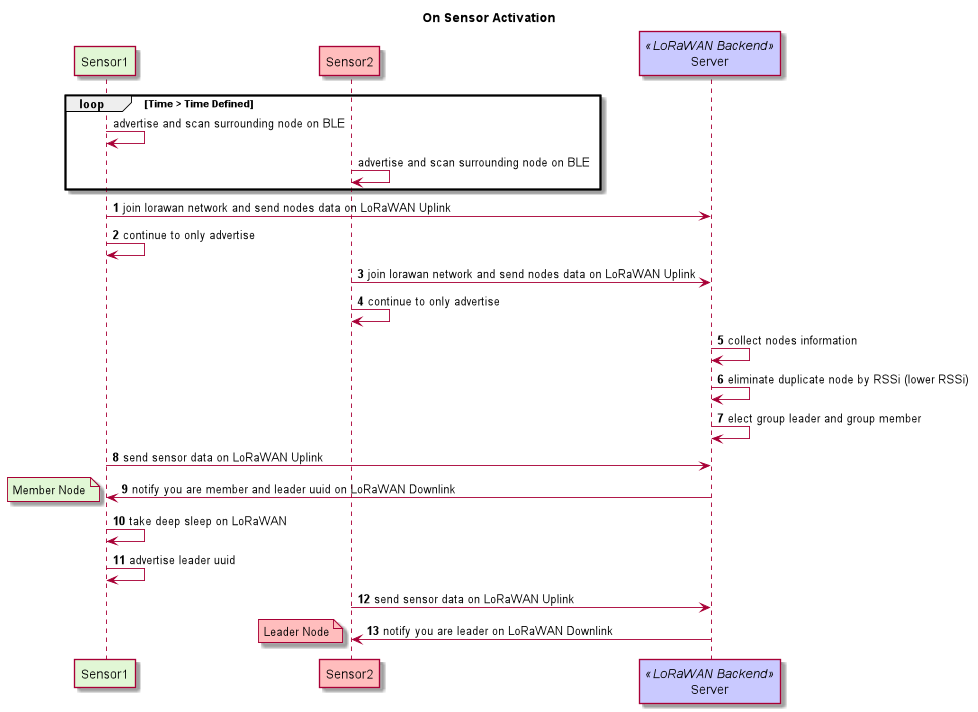
\includegraphics[width=14cm]{figures/グループ化_センサ起動時.png}
    \caption{グループ化の通信方式}
    \label{fig:group_on_activation}
    \end{center}
\end{figure}